\section{Sentiment Analysis}

The last analysis I performed on the dataset was a sentiment analysis using the \textit{transformers} library from Hugging Face.

Originally I wanted to use \textit{MilaNLProc/feel-it-italian-emotion}\footnote{\url{https://huggingface.co/MilaNLProc/feel-it-italian-emotion}}, a model trained on the FEEL-IT corpus, made of Italian Twitter posts annotated with four basic emotions: anger, fear, joy, sadness.
Unfortunately, at the time of writing the model's tokenizer is not compatible with any Python version I tried. 

I opted for one of the most popular free models, \textit{nlptown/bert-base-multilingual-uncased-sentiment}\footnote{\url{https://huggingface.co/nlptown/bert-base-multilingual-uncased-sentiment}.}, a bert-base-multilingual-uncased model fine-tuned for sentiment analysis on product reviews in six languages: English, Dutch, German, French, Spanish, and Italian. It predicts the sentiment as a number of stars (between 1 and 5).

I used a \textit{pipeline} from the \textit{transformers} library, and I ran the classifier on 512 tokens at a time, which is BERT's maximum input length. 

The classifier returns two results: a label (between 1 and 5, as in \textit{"4 stars"}), and a score, which represents how confident the model is about the label itself. For example, if a piece of text is labelled as four stars with a score of 0.5, the model is only 50\% sure that that text should be labelled as four stars.

To make comparison easier, I aggregated labels and scores with the following formula: 

\begin{center}
    $\frac{\text{amount of stars}*score}{5}$

\end{center}

Lastly, I appended the lists with all the scores to the original datasets.

A code example can be seen in listing \ref{code:sentiment}. De Gasperi's median aggregated sentiment is $0.265$, while Meloni's median aggregated sentiment is $0.379$. A visualization of the aggregated sentiment can be seen in figure \ref{fig:sentiment_comparison}. The samples are picked at random.


\begin{lstlisting}[language={python},label={code:sentiment}, caption={Example code for a function that calculates the sentiment score for each piece of text.}]
sentiment_classifier = pipeline(
    "text-classification",
    model="nlptown/bert-base-multilingual-uncased-sentiment",
    device=0  # GPU
)

sentiment_results = sentiment_classifier(
    texts,                  # list with all speeches
    batch_size=batch_size, 
    truncation=True, 
    max_length=512          # BERT max input length
)

df['sentiment_aggregated'] = [
    (int(res['label'].split()[0]) * res['score']) / 5 
    for res in sentiment_results
]
return df
\end{lstlisting}

\begin{figure}[h]
  \centering
  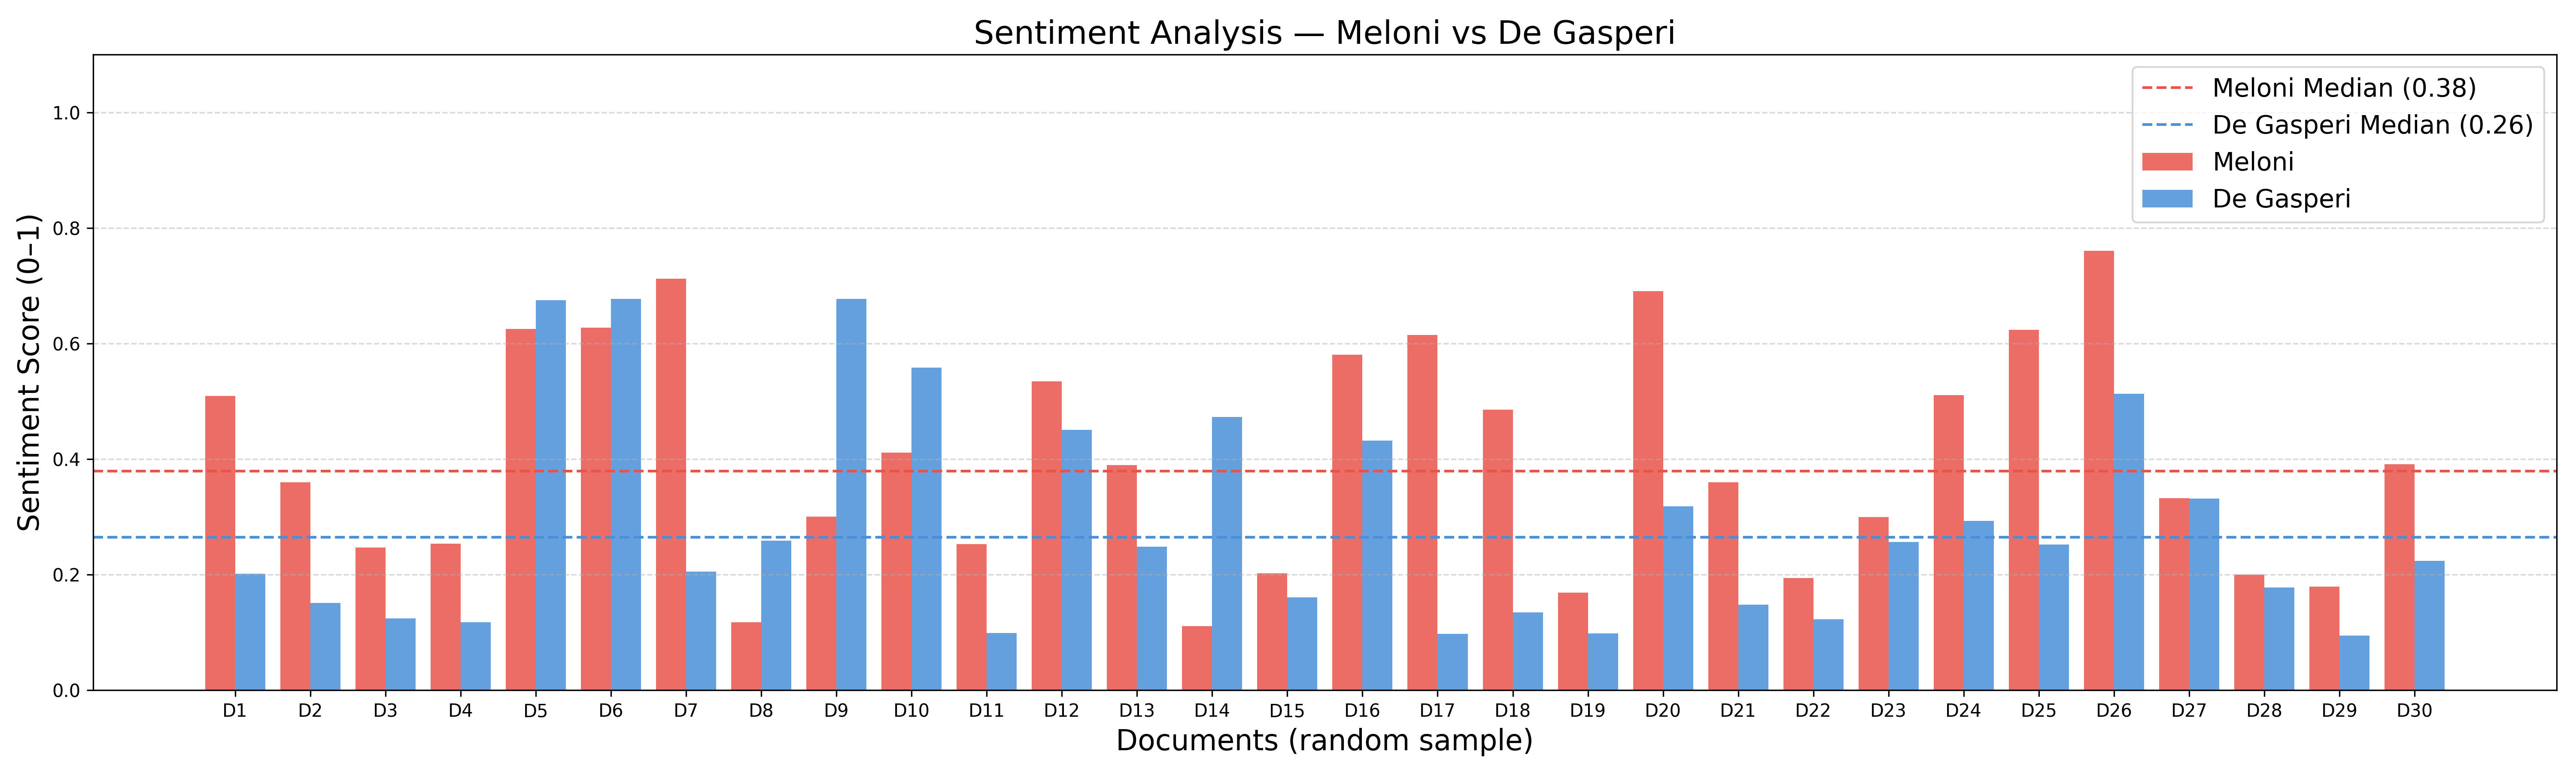
\includegraphics[width=\linewidth]{images/sentiment_comparison_30.png}
  \caption{Aggregated sentiment for 60 different speeches (30 for each Prime Minister), randomly sampled. The Y-axis reports the sentiment score (range between zero and one), while on the X-axis there are the relative IDs for the pairs of speeches. Each pair of speeches is represented by a two vertical bars (one red for Meloni, one blue for De Gasperi). Bar height represents their respective speech's aggregated sentiment score. The median scores for both Prime Ministers are shown by the two horizontal dotted lines.}
  \label{fig:sentiment_comparison}
\end{figure}

\subsection{Limitations and Future Work}

The model used to perform the sentiment analysis was designed to classify product reviews, and it struggled with long political speeches. This is evident from the sentiment scores (shown in table \ref{tab:sentiment_score}), where the model's confidence in its classifications is around 40\%.

It would be interesting to perform a sentiment analysis on the same corpus with a model trained on, for example, newspaper articles.

In future work, fine-tuning a model on labelled political speeches should produce better classification output.

\begin{table}[h]
    \centering
    \caption{Mean and median sentiment scores of the sentiment analysis for Meloni and De Gasperi.}
    \label{tab:sentiment_score}
    \begin{tabular}{lcc}
        \toprule
        \textbf{Metric} & \textbf{Meloni} & \textbf{De Gasperi} \\
        \midrule
        Mean Sentiment Score   & 0.4636 & 0.4068 \\
        Median Sentiment Score & 0.4692 & 0.3627 \\
        \bottomrule
    \end{tabular}
\end{table}